\documentclass[a4paper,11pt]{article}

\usepackage{amsfonts}
\usepackage{amsmath}
\usepackage{amssymb}
\usepackage{graphicx}

\usepackage[utf8]{inputenc}
%\usepackage[cp1250]{inputenc}
\usepackage[polish]{babel}
\usepackage[T1]{fontenc}

%----------------------
\def\\{\hfill\break}


%----------------------
\title{Projekt Egzaminacyjny}
\author{Jan Milewczyk}
\date{Spółka DIGITREE (DTR)}

\begin{document}

\maketitle

\section{Wstęp}
Digitree to polska spółka technologiczna specjalizująca się w kompleksowych rozwiązaniach z zakresu digital marketingu i wsparcia sprzedaży online.


\section{Analiza log-zwrotów spółki DIGITREE}

\subsection{Spółka DIGITREE}
Poniżej przedstawiam wykres kursów zamknięcia wybranej spółki

\centerline{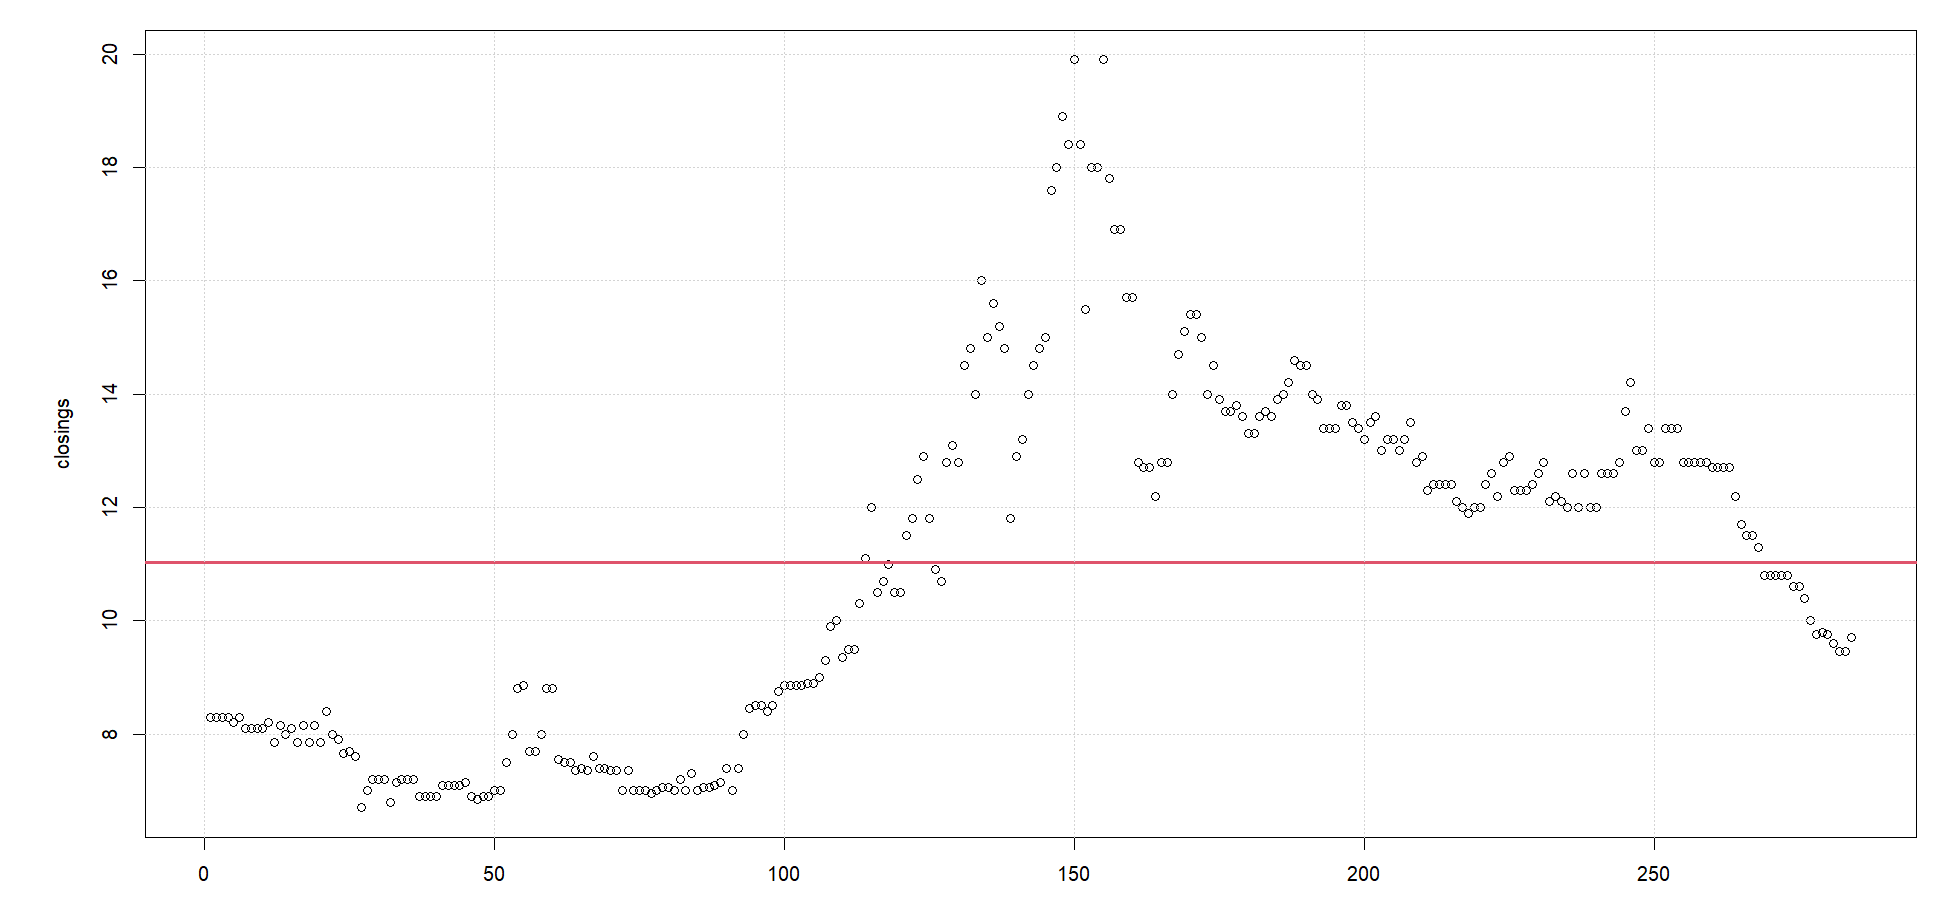
\includegraphics[width=14cm]{zamkniecie.png}}

Poniżej przedstawiam wykres log-zwrotów wybranej spółki

\centerline{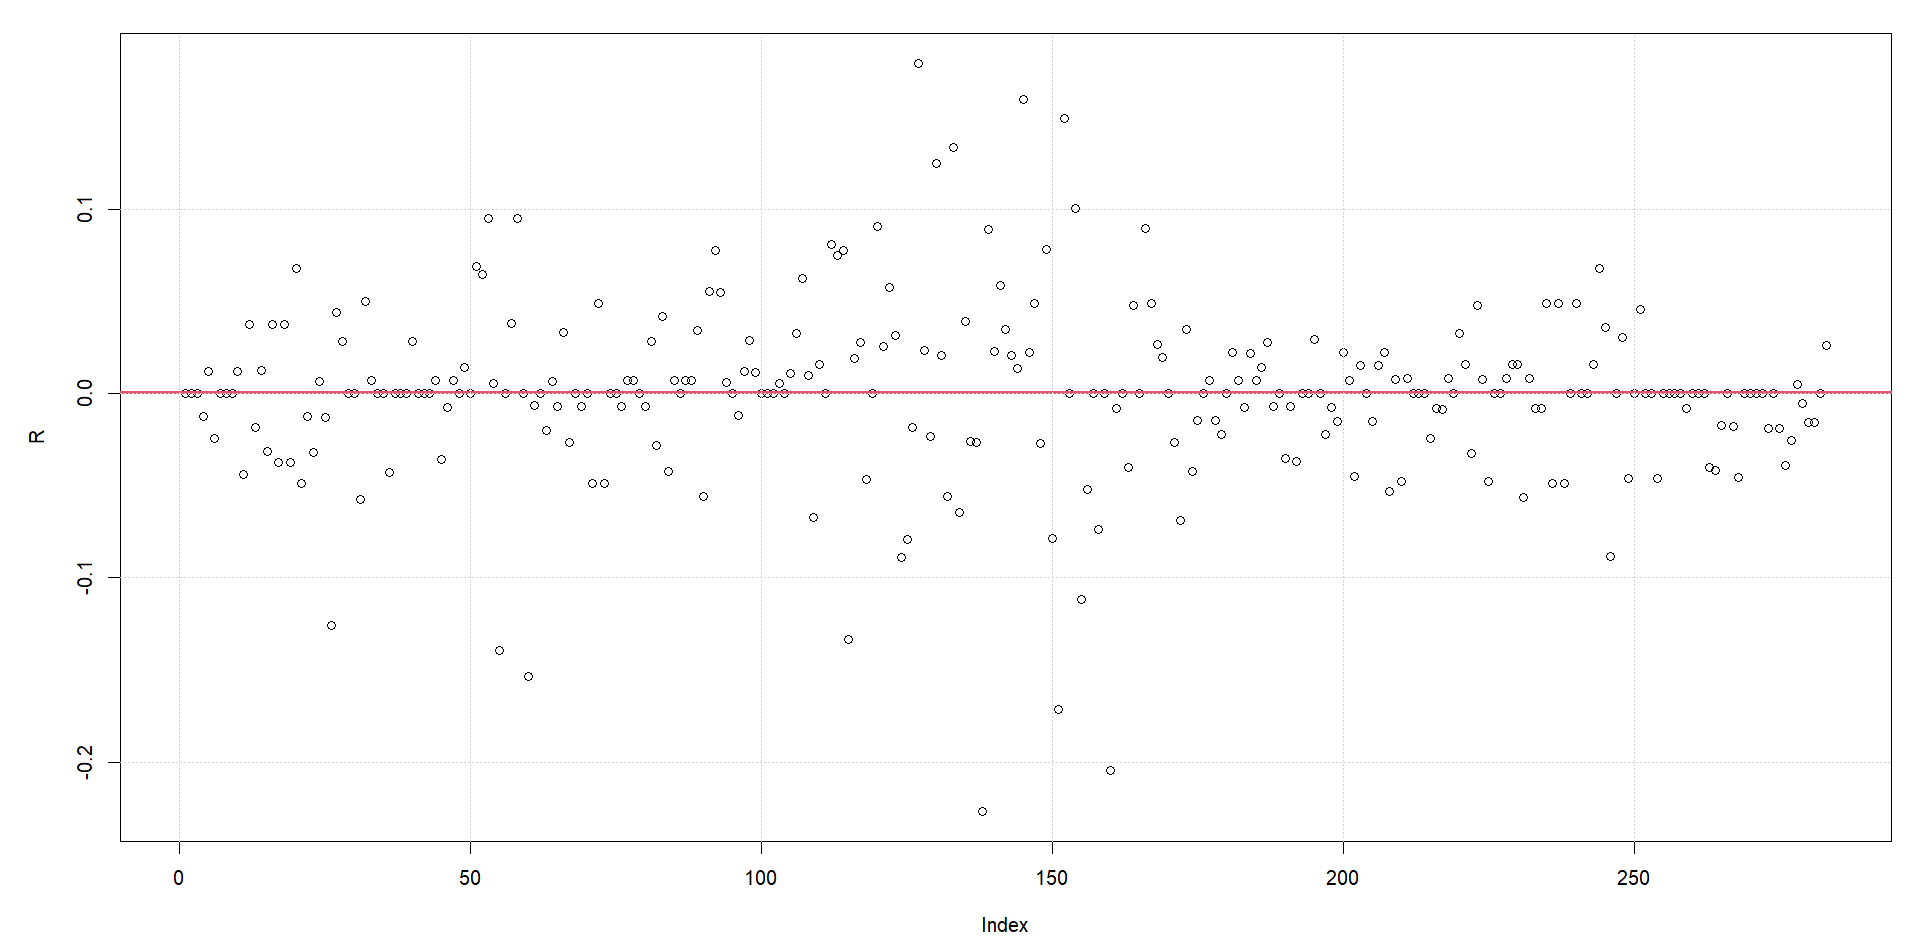
\includegraphics[width=14cm]{logzwroty.png}}

\subsection{Podstawowa analiza statystyczna log-zwrotów}

Wartości log-zwrotów zostały obliczone jako różnice logarytmiczne dziennych kursów zamknięcia. Poniżej przedstawiono podstawowe statystyki log-zwrotów:
\begin{itemize}
    \item Średnia log-zwrotów: $\overline{x}_n = 0.0005507787$
    \item Wariancja log-zwrotów: $s^2_n = 0.0022445$
    \item Odchylenie standardowe log-zwrotów: $s_n = 0.04737616$
\end{itemize}

\begin{table}[h!]
\centering
\caption{Estymacja parametrów log-zwrotów}
\begin{tabular}{|c|c|c|c|c|c|}
\hline
$\overline{x}_n$ & $s^2_n$ & $s_n$ & $q(5\%)$ & $q(50\%)$ & $q(95\%)$ \\ \hline
0.0005507787 & 0.0022445 & 0.04737616 & -0.06694173 & 0.00000000 & 0.07764551 \\ \hline
\end{tabular}
\end{table}

Kwantyle 5%, 50%, i 95% przedstawiają odpowiednio wartości, poniżej których znajduje się odpowiednio 5%, 50%, i 95% log-zwrotów. Na przykład, wartość kwantyla 5% oznacza, że 5% log-zwrotów jest mniejszych od -0.0669.

\subsection{Histogram log-zwrotów z zaznaczoną średnią i kwantylami}

Poniżej zamieszczono histogram log-zwrotów z zaznaczonymi wartościami średniej oraz kwantyli 5%, 50% i 95%.

\centerline{\includegraphics[width=14cm]{histogram_logzwroty.png}}

\subsection{Dystrybuanta empiryczna log-zwrotów}

Estymacja dystrybuanty empirycznej dla log-zwrotów została przeprowadzona przy użyciu wzoru empirycznej dystrybuanty $F_n(x)$. Wykres dystrybuanty empirycznej log-zwrotów znajduje się poniżej.

\centerline{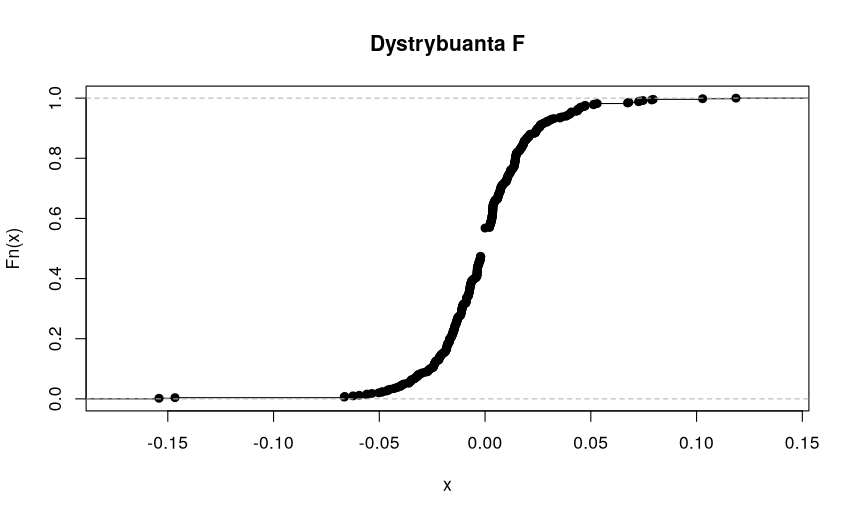
\includegraphics[width=14cm]{dystrybuanta.png}} 

\section{Analiza dobroci dopasowania rozkładów}

\subsection{Estymacja parametrów rozkładu normalnego i t-Studenta}

Parametry rozkładu normalnego i t-Studenta zostały wyestymowane przy użyciu estymatora największej wiarygodności (MLE):
\begin{itemize}
    \item Rozkład normalny: średnia = 0.0005507787, odchylenie standardowe = 0.0472923802
    \item Rozkład t-Studenta: liczba stopni swobody = 307.2041
\end{itemize}

\subsection{Wykresy diagnostyczne}

Poniżej przedstawiono wykresy diagnostyczne dla dopasowania rozkładów normalnego i t-Studenta do danych log-zwrotów, umożliwiające ocenę jakości dopasowania.

\centerline{\includegraphics[width=14cm]{dopasowanie_gestosc.png}}
\centerline{\includegraphics[width=14cm]{dopasowanie_kwantyle.png}} 
\centerline{\includegraphics[width=14cm]{dopasowanie_dystrybuanta.png}}
\centerline{\includegraphics[width=14cm]{dopasowanie_pradopodobienstwo.png}} 

\subsection{Ocena dopasowania rozkładów}

Na podstawie wykresów diagnostycznych oraz statystyk dopasowania:
\begin{itemize}
    \item Statystyki dla rozkładu normalnego: KS = 0.1561, CM = 1.8659, AD = 9.3673, AIC = -919.9766, BIC = -912.6857
    \item Statystyki dla rozkładu t-Studenta: KS = 0.4424, CM = 21.0334, AD = 99.0999, AIC = 523.2149, BIC = 526.8603
\end{itemize}

Wyniki sugerują, że rozkład normalny lepiej dopasowuje się do danych log-zwrotów niż rozkład t-Studenta. Wybór rozkładu normalnego uzasadniają niższe wartości AIC i BIC oraz lepsze dopasowanie na wykresach diagnostycznych.

\subsection{Test hipotezy o równości rozkładów}

Przeprowadzono test hipotezy o równości rozkładów dla wybranego rozkładu normalnego, wykorzystując statystykę Kolmogorova-Smirnova (KS). Wyniki testu przedstawiono poniżej:

\begin{itemize}
    \item \textbf{Statystyka testowa \( D \):} Obliczona wartość wynosi \( D = 0.1561313 \). Statystyka \( D \) mierzy maksymalną różnicę pomiędzy dystrybuantą empiryczną danych a teoretyczną dystrybuantą rozkładu normalnego. Wysoka wartość \( D \) wskazuje na większą różnicę, co może sugerować, że dane nie pochodzą z badanego rozkładu.
    \item \textbf{P-wartość (\( p \)):} Obliczona p-wartość wynosi \( p = 0 \). Oznacza to, że przy założeniu prawdziwości hipotezy zerowej, prawdopodobieństwo uzyskania tak dużej lub większej różnicy \( D \) wynosi praktycznie zero. W rezultacie, hipoteza zerowa o zgodności rozkładu danych z rozkładem normalnym zostaje odrzucona na dowolnym poziomie istotności.
\end{itemize}

\textbf{Interpretacja:}
\begin{itemize}
    \item Obliczona wartość statystyki \( D \) sugeruje, że istnieją istotne różnice pomiędzy rozkładem danych a teoretycznym rozkładem normalnym. 
    \item Niska p-wartość (\( p = 0 \)) wskazuje, że te różnice są statystycznie istotne. Oznacza to, że dane najprawdopodobniej nie pochodzą z badanego rozkładu normalnego.
\end{itemize}


\end{document}